\documentclass{../../note}

\usepackage{amsthm}
\usepackage{pgfplots}
\pgfplotsset{compat=1.18}
\newtheorem{example}{Example}
\usepackage{xcolor} % For colored text
\usepackage{tikz}
\usetikzlibrary{shapes,arrows,positioning,fit,calc,matrix,decorations.pathreplacing}
\usepackage{algorithm}
\usepackage{algpseudocode}
\usepackage{listings}
\lstset{
  basicstyle=\ttfamily\small,
  keywordstyle=\color{blue},
  commentstyle=\color{green!60!black},
  stringstyle=\color{purple},
  numbers=left,
  numberstyle=\tiny,
  numbersep=5pt,
  breaklines=true,
  frame=single,
}

\title{Exam 01}
\author{isomo}
\setlength{\parindent}{0em}
\begin{document}

\fontsize{12pt}{14.4pt}\selectfont

\maketitle
\tableofcontents
\newpage

依据考纲,数据结构和数据库分数,各占50\%,以下为大题的考点:

\subsection{数据结构}
在数据结构上,容易考的主要有树的前中序遍历,哈夫曼树的构造,图到树的转化。代码主要在二分查找,插入、选择、冒泡排序。

\subsection{数据库}
数据库主要考的是关系E-R模型,主码判定,SQL语句。

\noindent\rule{\textwidth}{1pt}

\section{数据结构}

\subsection{树的遍历}

\begin{example}
给定一棵二叉树的前序遍历序列为 ABDEGCFH,中序遍历序列为 DBGEACFH,请:
\begin{enumerate}
  \item 画出这棵二叉树
  \item 写出这棵二叉树的后序遍历序列
  \item 用C语言实现该二叉树的构建和后序遍历
\end{enumerate}
\end{example}

\subsection{哈夫曼树}

\begin{example}
给定以下字符及其出现频率:A(5), B(29), C(7), D(8), E(14), F(23), G(3), H(11)
\begin{enumerate}
  \item 构造哈夫曼树
  \item 给出每个字符的哈夫曼编码
  \item 计算平均编码长度
\end{enumerate}
\end{example}

\subsection{图与树的转换}

\begin{example}
给定如下的无向图G:
\begin{center}
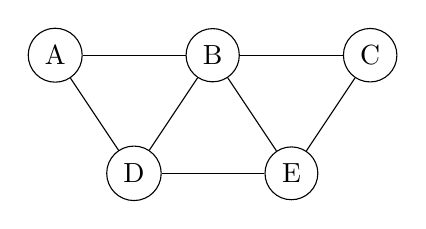
\begin{tikzpicture}
    \node[circle,draw] (A) at (0,0) {A};
    \node[circle,draw] (B) at (2,0) {B};
    \node[circle,draw] (C) at (4,0) {C};
    \node[circle,draw] (D) at (1,-1.5) {D};
    \node[circle,draw] (E) at (3,-1.5) {E};

    \draw (A) -- (B);
    \draw (B) -- (C);
    \draw (A) -- (D);
    \draw (B) -- (D);
    \draw (B) -- (E);
    \draw (C) -- (E);
    \draw (D) -- (E);
\end{tikzpicture}
\end{center}

\begin{enumerate}
  \item 从顶点A开始,构造该图的深度优先生成树
  \item 从顶点A开始,构造该图的广度优先生成树
\end{enumerate}
\end{example}

\subsection{查找与排序}

\begin{example}
请实现二分查找算法,并分析其时间复杂度。
\begin{lstlisting}[language=C]
int binarySearch(int arr[], int n, int key) {
    // 请完成代码
}
\end{lstlisting}
\end{example}

\begin{example}
给定数组 [64, 34, 25, 12, 22, 11, 90]:
\begin{enumerate}
  \item 用冒泡排序对其进行排序,写出每一趟排序后的结果
  \item 用选择排序对其进行排序,写出每一趟排序后的结果
  \item 用插入排序对其进行排序,写出每一趟排序后的结果
\end{enumerate}
\end{example}

\begin{example}
请用C语言实现冒泡排序、选择排序和插入排序算法,并比较它们的时间复杂度和空间复杂度。
\begin{lstlisting}[language=C]
void bubbleSort(int arr[], int n) {
    // 请完成代码
}

void selectionSort(int arr[], int n) {
    // 请完成代码
}

void insertionSort(int arr[], int n) {
    // 请完成代码
}
\end{lstlisting}
\end{example}

\subsection{栈与队列应用}

\begin{example}
请用C语言实现一个栈,并利用该栈实现表达式求值算法。以下是一个简化版本,仅考虑整数、加减乘除运算和括号。
\begin{lstlisting}[language=C]
typedef struct {
    int data[100];
    int top;
} Stack;

int evaluateExpression(char* expression) {
    // 请完成代码
}
\end{lstlisting}
\end{example}

\begin{example}
使用队列实现二叉树的层序遍历。
\begin{lstlisting}[language=C]
typedef struct BiTNode {
    char data;
    struct BiTNode *lchild, *rchild;
} BiTNode, *BiTree;

void levelOrderTraversal(BiTree T) {
    // 请完成代码
}
\end{lstlisting}
\end{example}

\subsection{线性表操作}

\begin{example}
实现单链表的逆置操作。
\begin{lstlisting}[language=C]
typedef struct LNode {
    int data;
    struct LNode *next;
} LNode, *LinkList;

void reverseList(LinkList *L) {
    // 请完成代码
}
\end{lstlisting}
\end{example}

\begin{example}
给定一个有序链表,请删除链表中的重复元素,使每个元素只出现一次。
\begin{lstlisting}[language=C]
typedef struct LNode {
    int data;
    struct LNode *next;
} LNode, *LinkList;

void removeDuplicates(LinkList L) {
    // 请完成代码
}
\end{lstlisting}
\end{example}

\subsection{更多树的操作}

\begin{example}
给定二叉树的前序遍历序列为 GDAFEMHZ,中序遍历序列为 ADEFGHMZ。请:
\begin{enumerate}
  \item 画出该二叉树
  \item 计算该二叉树的深度
  \item 求出所有叶子节点
\end{enumerate}
\end{example}

\begin{example}
编写函数统计二叉树中度为2的结点个数。
\begin{lstlisting}[language=C]
typedef struct BiTNode {
    char data;
    struct BiTNode *lchild, *rchild;
} BiTNode, *BiTree;

int countNodes2Degree(BiTree T) {
    // 请完成代码
}
\end{lstlisting}
\end{example}

\subsection{图的应用}

\begin{example}
请用表示下图,使用Dijkstra算法描述从顶点A到其他各顶点的最短路径,计算过程。
\begin{center}
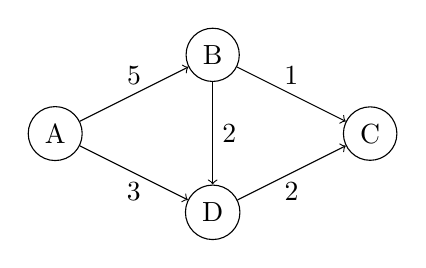
\begin{tikzpicture}
    \node[circle,draw] (A) at (0,0) {A};
    \node[circle,draw] (B) at (2,1) {B};
    \node[circle,draw] (C) at (4,0) {C};
    \node[circle,draw] (D) at (2,-1) {D};

    \draw[->] (A) -- node[above] {5} (B);
    \draw[->] (A) -- node[below] {3} (D);
    \draw[->] (B) -- node[above] {1} (C);
    \draw[->] (D) -- node[below] {2} (C);
    \draw[->] (B) -- node[right] {2} (D);
\end{tikzpicture}
\end{center}


\end{example}

\begin{example}
判断下图是否为一棵树,如果不是,给出理由;如果是,画出对应的树结构。
\begin{center}
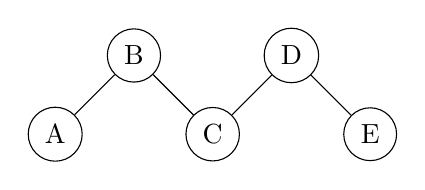
\begin{tikzpicture}
    \node[circle,draw] (A) at (0,0) {A};
    \node[circle,draw] (B) at (1,1) {B};
    \node[circle,draw] (C) at (2,0) {C};
    \node[circle,draw] (D) at (3,1) {D};
    \node[circle,draw] (E) at (4,0) {E};

    \draw (A) -- (B);
    \draw (B) -- (C);
    \draw (C) -- (D);
    \draw (D) -- (E);
\end{tikzpicture}
\end{center}
\end{example}

\subsection{高级排序算法}

\begin{example}
给定数组 [38, 27, 43, 3, 9, 82, 10],请演示快速排序的详细过程,写出每一趟排序后的结果。
\end{example}

\begin{example}
请用C语言实现快速排序算法。
\begin{lstlisting}[language=C]
void quickSort(int arr[], int low, int high) {
    // 请完成代码
}
\end{lstlisting}
\end{example}

\section{数据库}

\subsection{关系模型与E-R图}

\begin{example}
将下述E-R图转换为关系模式,并标明主码、外码。

\begin{center}
\begin{tikzpicture}
    % 实体
    \node[rectangle,draw,minimum width=2cm,minimum height=1cm] (student) {学生};
    \node[rectangle,draw,minimum width=2cm,minimum height=1cm] (course) at (6,0) {课程};
    \node[diamond,draw,minimum width=2cm,minimum height=1cm] (sc) at (3,0) {选修};

    % 属性
    \node[ellipse,draw] (sno) at (-2,1.5) {学号};
    \node[ellipse,draw] (sname) at (-1,2.5) {姓名};
    \node[ellipse,draw] (ssex) at (0,3) {性别};
    \node[ellipse,draw] (sdept) at (1,2.5) {系别};

    \node[ellipse,draw] (cno) at (5,2.5) {课程号};
    \node[ellipse,draw] (cname) at (6,3) {课程名};
    \node[ellipse,draw] (credit) at (7,2.5) {学分};

    \node[ellipse,draw] (grade) at (3,2) {成绩};

    % 连线
    \draw (student) -- (sc);
    \draw (sc) -- (course);
    \draw (student) -- (sno);
    \draw (student) -- (sname);
    \draw (student) -- (ssex);
    \draw (student) -- (sdept);
    \draw (course) -- (cno);
    \draw (course) -- (cname);
    \draw (course) -- (credit);
    \draw (sc) -- (grade);

    % 多重性标记
    \node at (1.7,0.2) {1};
    \node at (4.3,0.2) {n};
\end{tikzpicture}
\end{center}
\end{example}

\begin{example}
根据以下描述,画出E-R图,然后转换为关系模式:

一个图书管理系统需要管理图书馆的图书和读者信息。每本图书有唯一的编号、书名、作者、出版社、出版日期和价格。每位读者有唯一的借书证号、姓名、性别、单位和电话。读者可以借阅多本图书,每本图书也可以被多位读者借阅(但不能同时)。系统需要记录借阅日期和归还日期。
\end{example}

\begin{example}
给定关系模式 R(A,B,C,D,E,F),其中函数依赖集为:
\begin{align*}
F = \{A \rightarrow B, BC \rightarrow D, AE \rightarrow F, F \rightarrow A\}
\end{align*}

\begin{enumerate}
  \item 求出 R 的所有候选码
  \item 判断该关系模式属于哪种范式
\end{enumerate}
\end{example}

\begin{example}
给定关系模式 S(A,B,C,D,E),其中函数依赖集为:
\begin{align*}
F = \{A \rightarrow B, B \rightarrow C, D \rightarrow E, C \rightarrow D\}
\end{align*}

\begin{enumerate}
  \item 求出 S 的候选码
  \item 该关系模式满足哪一级范式?
\end{enumerate}
\end{example}


\subsection{SQL语句}

\begin{example}
假设有以下关系模式:
\begin{align*}
&\text{学生}: \text{Student}(\underline{\text{Sno}}, \text{Sname}, \text{Ssex}, \text{Sage}, \text{Sdept})\\
&\text{课程}: \text{Course}(\underline{\text{Cno}}, \text{Cname}, \text{Cpno}, \text{Ccredit})\\
&\text{学生选课}: \text{SC}(\underline{\text{Sno}}, \underline{\text{Cno}}, \text{Grade})
\end{align*}

请用SQL语句完成以下操作:
\begin{enumerate}
  \item 查询计算机系(CS)年龄在20岁以下的学生的学号和姓名
  \item 查询选修了课程名为"数据库"的学生学号和成绩
  \item 查询没有选修任何课程的学生姓名
  \item 查询选修了全部课程的学生姓名
\end{enumerate}
\end{example}

\begin{example}
假设有以下关系模式:
\begin{align*}
&\text{部门}: \text{Department}(\underline{\text{Dno}}, \text{Dname}, \text{Dlocation})\\
&\text{员工}: \text{Employee}(\underline{\text{Eno}}, \text{Ename}, \text{Esalary}, \text{Dno})\\
&\text{项目}: \text{Project}(\underline{\text{Pno}}, \text{Pname}, \text{Budget}, \text{Dno})\\
&\text{员工参与项目}: \text{Works\_on}(\underline{\text{Eno}}, \underline{\text{Pno}}, \text{Hours})
\end{align*}

请用SQL语句完成以下查询:
\begin{enumerate}
  \item 查询月薪超过3000元的员工姓名及其部门名称
  \item 查询参与了名为"数据库开发"项目的员工姓名及工作时间
  \item 查询平均月薪最高的部门编号、名称及平均月薪
  \item 查询至少参与了3个项目的员工姓名
  \item 查询没有员工参与的项目名称
\end{enumerate}
\end{example}

\begin{example}
针对上述学生-课程关系模式,编写SQL语句完成以下操作:
\begin{enumerate}
  \item 将"数据库"课程的学分增加1学分
  \item 删除没有选修任何课程的学生记录
  \item 创建一个新表存储各系的学生人数
  \item 为Student表的Sage字段添加检查约束,要求年龄在16到30之间
\end{enumerate}
\end{example}

\end{document}
